\chapter{Measurements}
\section{Narrow Band Transmission}
\label{sec:res_450}

First a relatively narrow signal transmitting at only a quarter
of the maximal symbol rate was build and analyzed to show some basic
properties of the system and to show what the best achievable
\gls{EVM} values are. \\

As receiver architecture, the Quadrature Intermediate Frequency Sub-Nyquist
Sampling Receiver as described in \secref{sec:rx_2} is used with the difference
that the signal bandwith is only $B = 450 MHz$. All the other properties are listed
in \tblref{tab:res_450}. \\

\begin{table}[h]
  \centering
  \begin{tabular}{|l|r@{}l@{~}l|}
    \hline
    $f_{\text{TX IF}}$ & 2&.9&GHz \\ \hline
    $f_{\text{TX LO}}$ & 57&.5&GHz \\ \hline
    $f_{\text{RX LO}}$ & 58&.2&GHz \\ \hline
    $f_{\text{RX IF}}$ & 2&.2&GHz \\ \hline
    $f_c$            & 60&.4&GHz \\ \hline
    Signal Bandwidth B & 0&.45&GHz \\ \hline
    Sample Rate $f_s$ & 1&.8&GHz \\ \hline
  \end{tabular}
  \caption{Properties of Narrow Band Transmission System}
  \label{tab:res_450}
\end{table}

\subsection{Measurement Setup and RF System Analysis}
A block diagram providing an overview of the test setup,
used for all following measurements, can be found in \figref{fig:res_450_bd}. \\

\begin{figure}[p]
  \centering
  %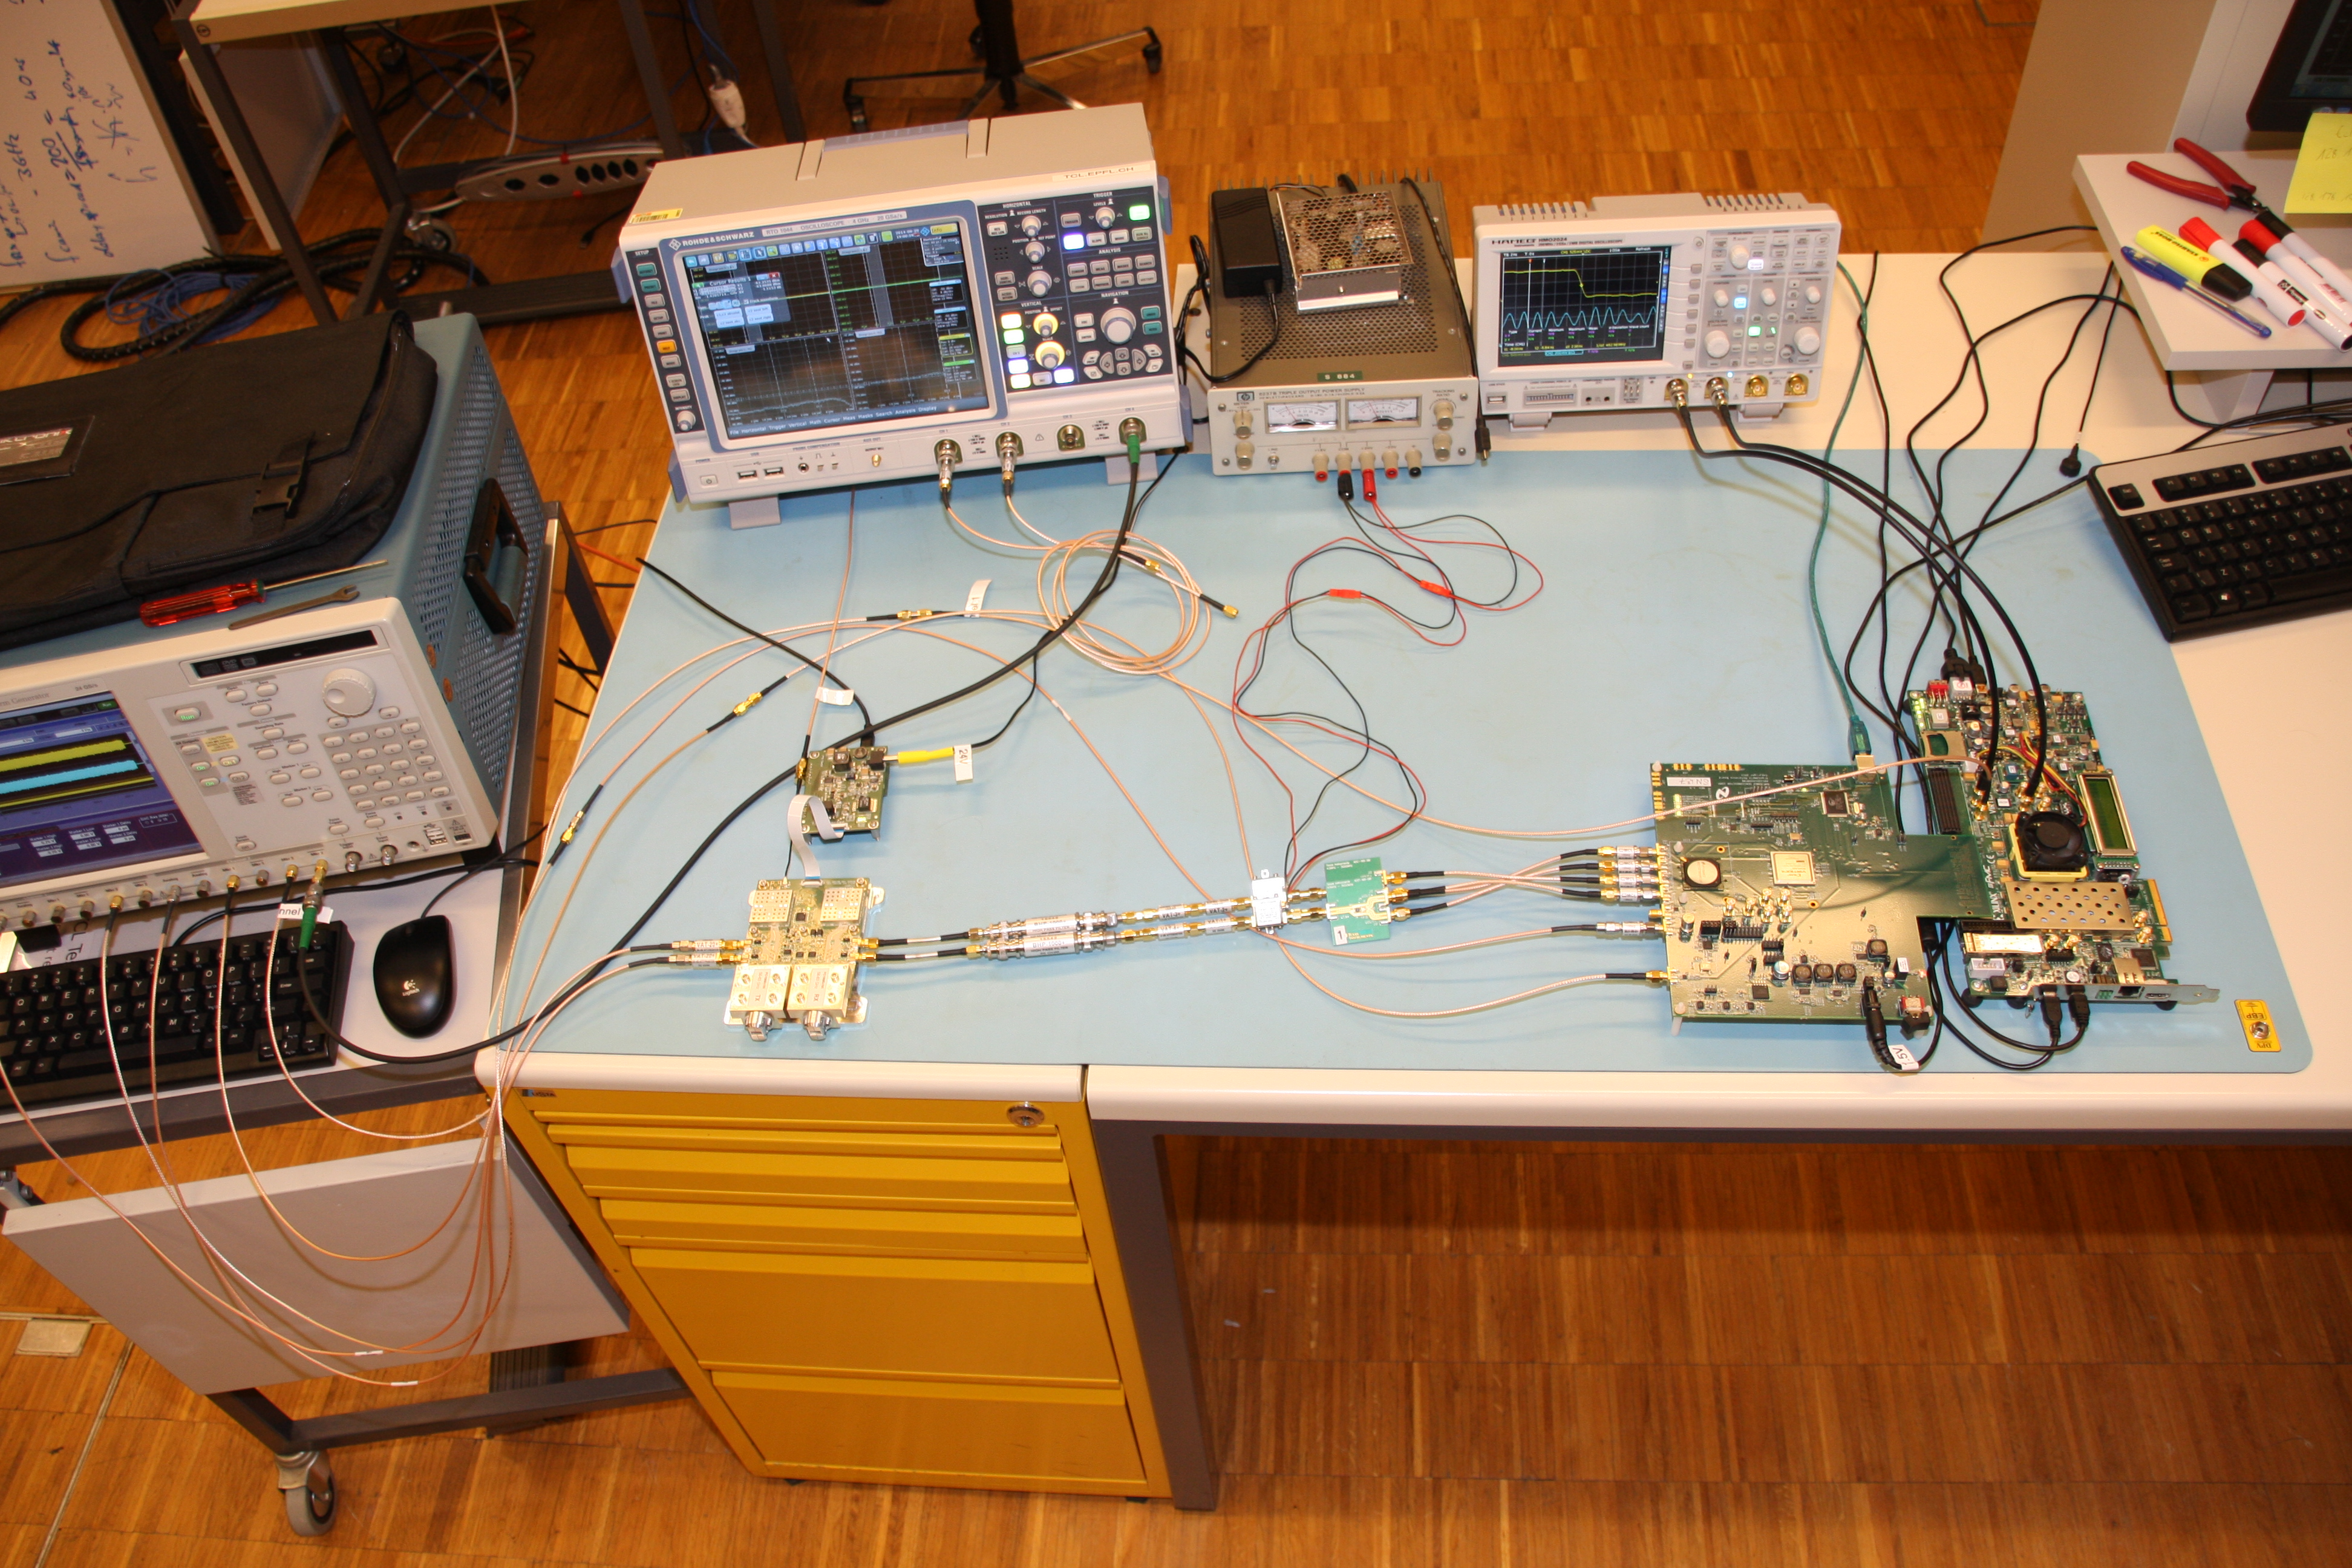
\includegraphics[width=\textwidth]{pictures/res_450_setup}
  \caption{Block Diagram of the Narrow Band Transmission Setup}
  \label{fig:res_450_bd}
\end{figure}
\todo{draw block diagram}

\begin{figure}[p]
  \centering
  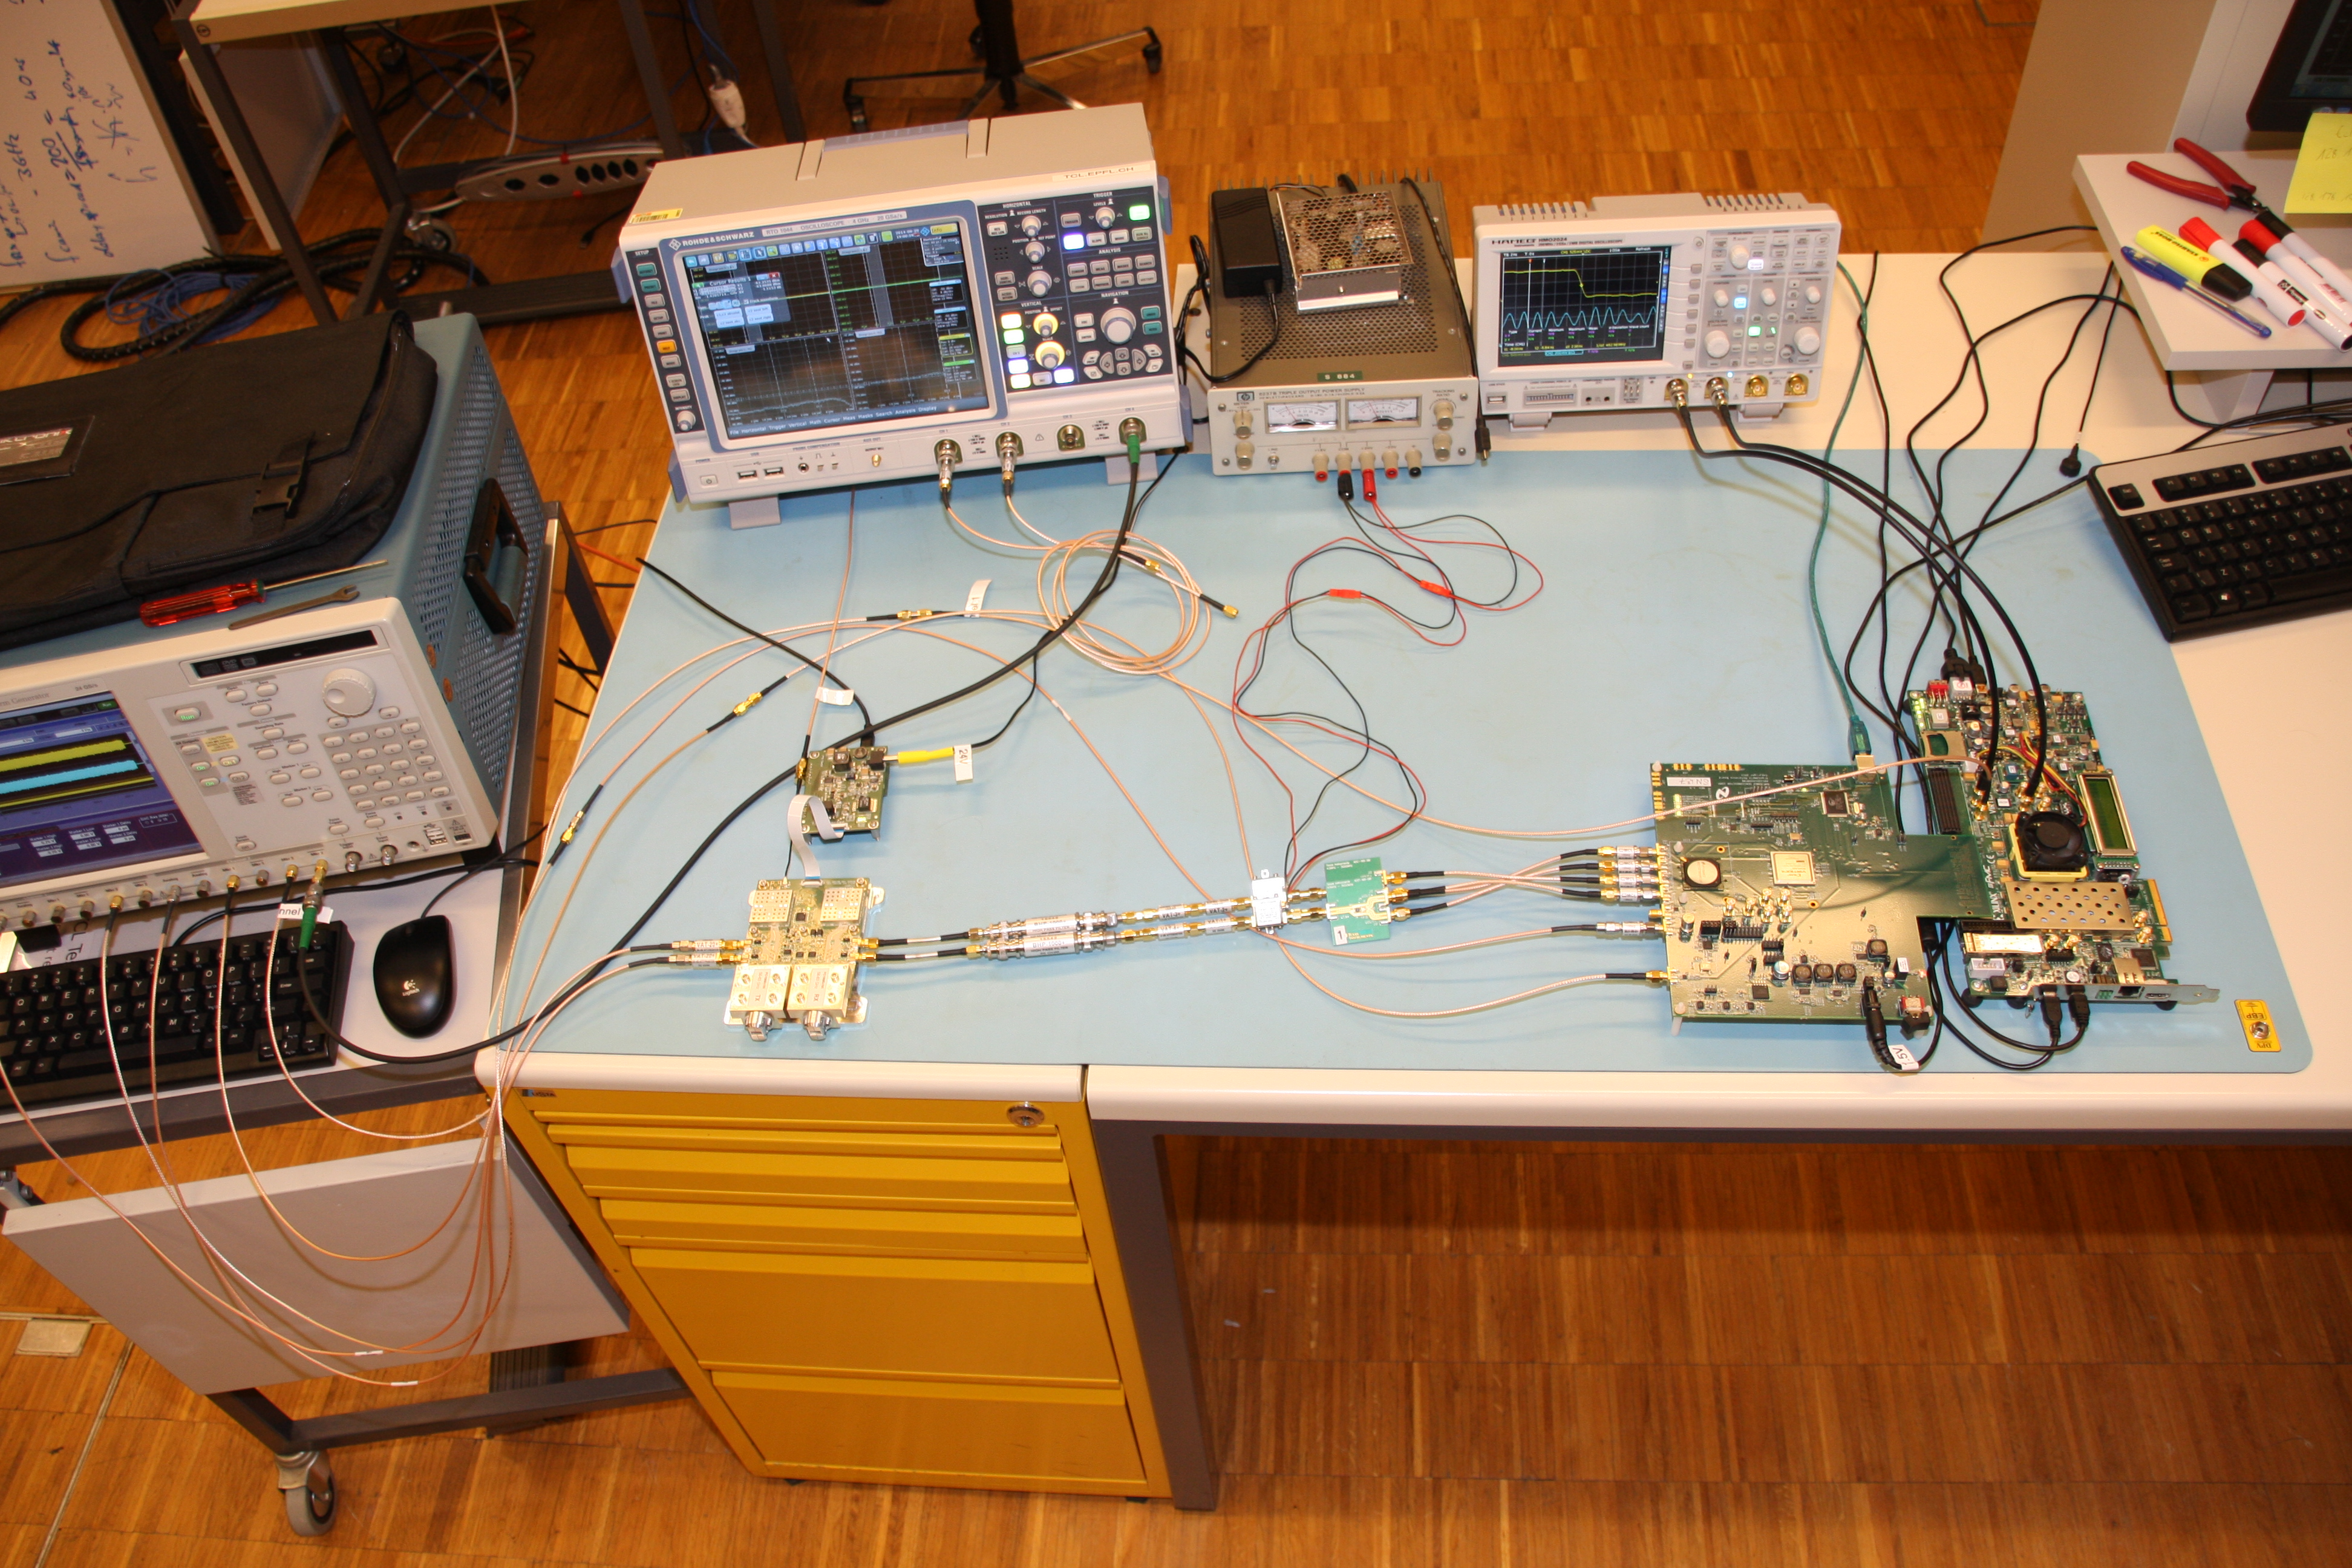
\includegraphics[width=\textwidth]{pictures/res_450_setup}
  \caption{Picture of the Narrow Band Transmission Setup}
  \label{fig:res_450_pic}
\end{figure}

\subsubsection{Matlab}
The Matlab script was configured such that it generates the transmitt signal,
programs the \gls{AWG}, reads the data acquired by the \gls{FPGA},
runs the receiver code and finally generets reports and figures. \\
The configuration file used for these tests can be found in
\appref{app:res_450_cnf}. \\

\subsubsection{\gls{AWG}}
The \gls{AWG} was configured to output the \gls{TX} \gls{IF} signal $i[k]$,
the sample clock for the \gls{ADC} as well as synchronization pulses to trigger
the \gls{FPGA} and oscillocope. It's configuration and port assignment
are shown in \tblref{tab:res_450_awg}.

It was noticed, that the used \gls{AWG} has some cross talk from
channel 1 marker 1 output to the channel 1 analog output. Therefor the
\gls{ADC} clock should always be output on marker 2 and not on marker 1.
For synchronization pulses, this is not an issue, since they are ware always
configured to give a 100 cycle wide positive pulse $> 100 \text{ns}$ before
the signal starts. \\

\begin{table}[h]
  \centering
  \begin{tabular}{|l|l|}
    \hline
    Sampling Rate & 10.8 GS/s \\ \hline
    Clock Source & Externals 10 MHz \\ \hline
    Analog Amplitude & 1 $\text{V}_{\text{pp}}$ \\ \hline
    Marker Amplitude CH1 Marker 1/2 & 0, 0.7 V \\ \hline
    Marker Amplitude CH2 Marker 1/2 & 0, 1.4 V \\ \hline
    \gls{DAC} resolution & 8 bit \\ \hline
    CH 1 & $i[k]$ \\ \hline
    CH 2 & $\mathcal{H}\{i[k]\}$ \\ \hline
    CH 1 Marker 1 & 0 \\ \hline
    CH 1 Marker 2 & 1.8 GHz \gls{ADC} sample clock \\ \hline
    CH 2 Marker 1 / 2 & Sync pulse before frame starts \\ \hline
  \end{tabular}
  \caption{Configuration and Port Assignment of \gls{AWG}}
  \label{tab:res_450}
\end{table}

An osilloscope plot (see \secref{sec:comp_osci}) of the generated
\gls{TX} \gls{IF} signal and it's \gls{FFT} can be found in
\figref{fig:res_450_awg_analog}.
The \gls{ADC} clock signal and the sync pulse are shown
in \figref{fig:res_450_awg_digital}. \\

\begin{figure}[p]
  \centering
  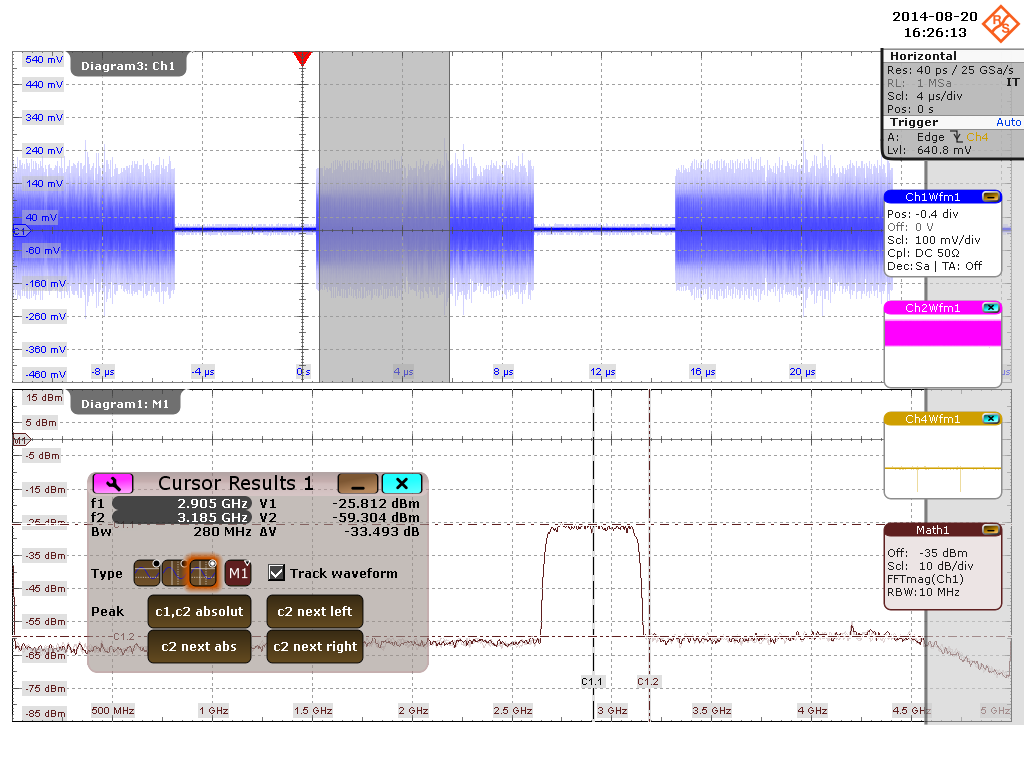
\includegraphics[width=\textwidth]{figures/osci/res_450_awg_analog}
  \caption{\gls{TX} \gls{IF} signal generated by the \gls{AWG}}
  \label{fig:res_450_awg_analog}
\end{figure}

\begin{figure}[p]
  \centering
  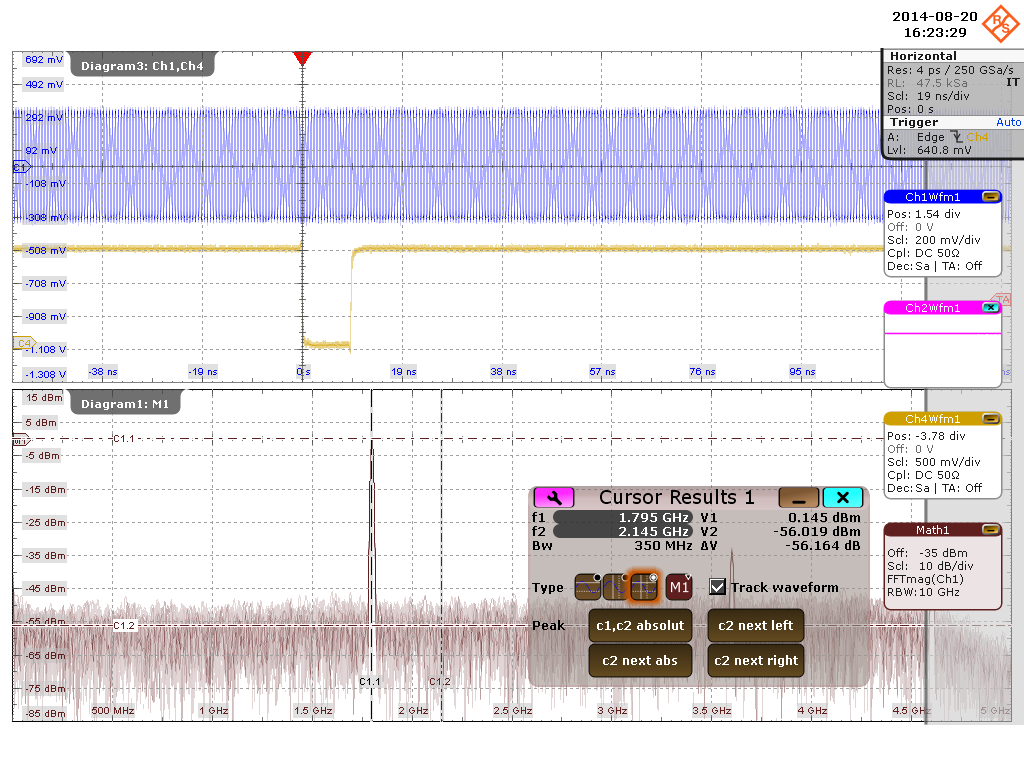
\includegraphics[width=\textwidth]{figures/osci/res_450_awg_digital}
  \caption{\gls{ADC} clock signal and sync pulse generated by the \gls{AWG}}
  \label{fig:res_450_awg_digital}
\end{figure}

\subsubsection{RF parts}
The two analog channels generated by the \gls{AWG} have a total signal
power of -9.28 dBm each \eqref{eq:res_450_awg_pwr}. These signals were
than attenuated by 20 dB to be below the 1-dB output compression point of 10 dBm
of the 60 GHz converters even at full gain of 40 dB. \\

\begin{align}
  10 \cdot \log_{10}\left(
  10^{-25.812 \;\text{dBm} / 10} \cdot
  \frac{450 \;\text{MHz}}{10 \;\text{MHz}}
  \right) \approx -9.28 \;\;\text{dBm}
  \label{eq:res_450_awg_pwr}
\end{align}

The same 60 GHz converter was used for transmission and reception and
configured as shown in \tblref{tab:res_450_sivers} (configuration script
see \appref{app:}).
A 10 MHz reference clock was fed from the \gls{AWG}.
An aluminium plate in a distance of about 15 cm was used as a reflector. \\

\begin{table}[h]
  \centering
  \begin{tabular}{|l|l|}
    \hline
    Reference Clock & external \\ \hline
    TX Oscillator Frequency & 57.5 GHz (0x038170) \\ \hline
    RX Oscillator Frequency & 58.2 GHz (0x038D60) \\ \hline
    TX Power & 0x80 \\ \hline
  \end{tabular}
  \caption{Configuration Parameters of 60 GHz Converter}
  \label{tab:res_450}
\end{table}

Both channels on the \gls{RX} side of the converer first connect to a
\gls{MC} BHP-1000+ high-pass filter. As we can see in \figref{fig:res_450_rx_if},
the \gls{TX} \gls{LO} leackage is attenuated by about 35 dB. Also the \gls{TX}
\gls{LSBand} signal (centered around 3.6 GHz) is about 17 dB weaker than
the desired \gls{TX} \gls{USBand} signal. This is due to the transmitter's
image rejection and the fact that the \gls{LSBand} signal is outside the
\gls{RF} specification of the converter. \\

\begin{figure}[p]
  \centering
  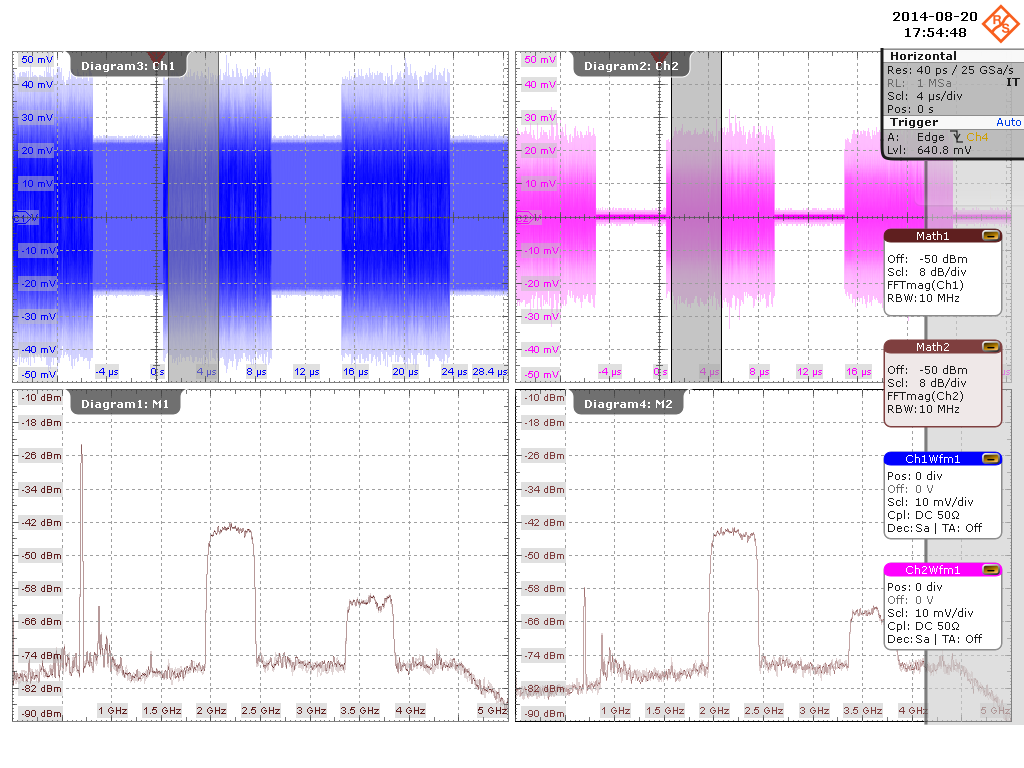
\includegraphics[width=\textwidth]{figures/osci/res_450_rx_if}
  \caption{Received \gls{IF} Signal before (left) and after (right) High-Pass Filter}
  \label{fig:res_450_rx_if}
\end{figure}p

Next the signal amplified by 12 dB to drive the \gls{ADC} input to about 70\%
as shown in \figref{fig:res_450_rx_amp}. \\

\begin{figure}[p]
  \centering
  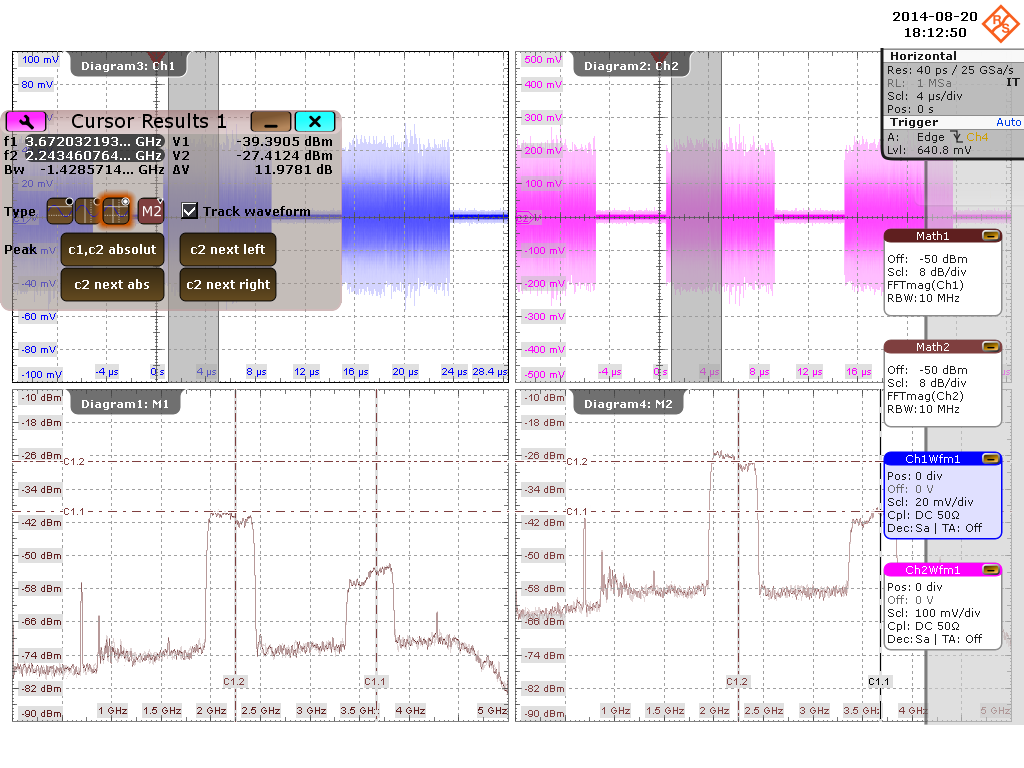
\includegraphics[width=\textwidth]{figures/osci/res_450_rx_amp}
  \caption{Received \gls{IF} Signal before (left) and after (right) the Amplifier}
  \label{fig:res_450_rx_amp}
\end{figure}

Finally the signal is converted to a differential signal using a ADC-WB-BB Balun
(\secref{sec:comp_balun}), passes a \gls{DC} block (\secref{sec:comp_dc_block})
and digitized by the \gls{ADC}. \\

The channel filter shown in \figref{fig:rx_2_bd} is therefor build using
the BHP-1000+ high-pass filter and the \gls{ADC} analog input bandwidth which
cuts of at about 2.8 GHz. \\

\subsection{Channel impulse response}
\label{sec:res_450_h}
First we should have a short look at the channel response of the simple
reflector. The estimated channel response using the Goaly estimator and a
1152 long \gls{CES} field is shown in \figref{fig:res_450_h}.
As we can see, there is one very distinctive peak confirming one single,
more or less flat, reflector. \\

\begin{figure}[p]
  \centering
  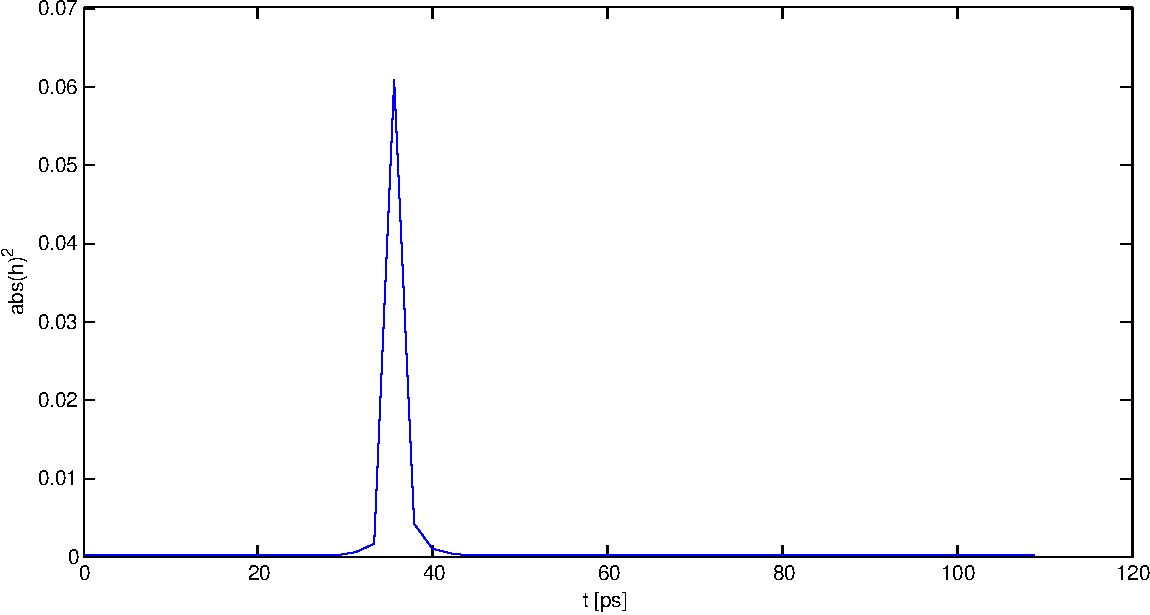
\includegraphics[width=0.8\textwidth]{figures/matlab/res_450_h}
  \caption{Channel response in Time Domain}
  \label{fig:res_450_h}
\end{figure}

\subsubsection{Root Mean Square Delay Spread}
\begin{align}
  \overline{\tau} &=\frac{\int_0^\infty\tau A_c(\tau)d\tau}{\int_0^\infty A_c(\tau)d\tau} \\
  \tau_{\text{rms}} &=\sqrt{\frac{\int_0^\infty(\tau-\overline{\tau})^2
      A_c(\tau)d\tau}{\int_0^\infty A_c(\tau)d\tau}}
\end{align}

\subsubsection{Delay Spread}
Root Mean Square Delay Spread is a nice statistical property of a channel.
When designing a receiver, it is more relevant though, that we now how many
samples have to be considered to capture enough energy of a symbol. \\

How much energy is significant, can be estimated depending on the \gls{SNR}
we want to achiev. The \gls{SNR} we want to reach depends on the modulation rate
we want to achiev. Therefor we first calculate the needed \gls{SNR} for
\gls{QAM}-256. \\

\todo{do SNR calculation and calc delay spread}
The delay spread $\approx $ 5 ps, which corresponds to about 7 symbols
at 450 MS/s and about 15 symbols at 1.8 GS/s. \\

\subsection{Error Vector Magnitude Measurements}
\begin{figure}[p]
  \centering
  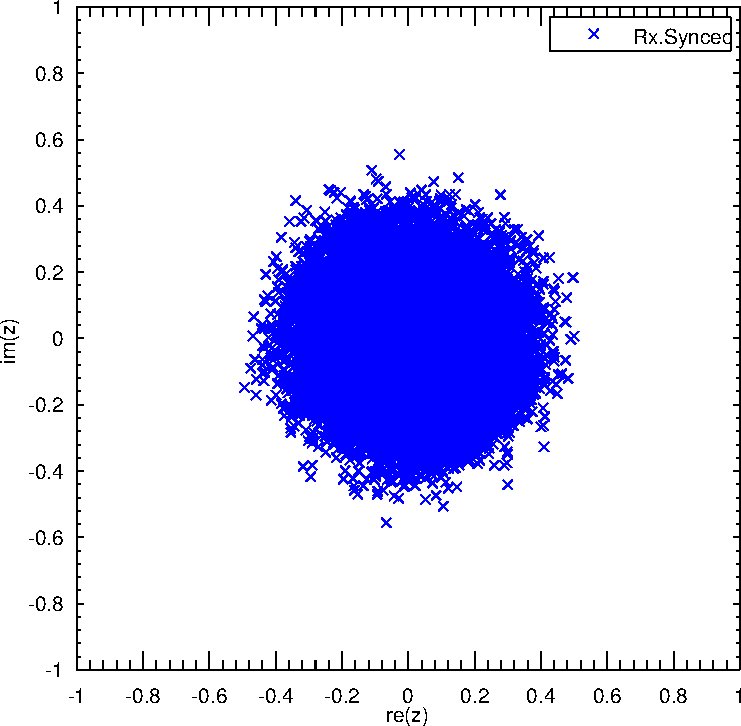
\includegraphics[width=0.6\textwidth]{figures/matlab/res_450_cp_synced}
  \caption{Received Data Points after Synchronization but before any Correction}
  \label{fig:res_450_cp_synced}
\end{figure}

\begin{figure}[p]
  \centering
  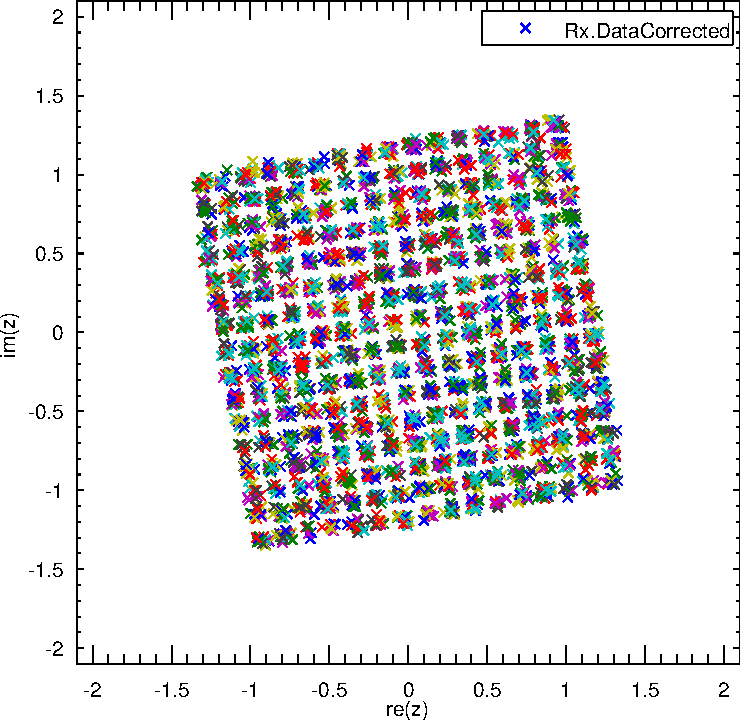
\includegraphics[width=0.6\textwidth]{figures/matlab/res_450_cp_corrected}
  \caption{Received Data Points after Correction (one color per data packet)}
  \label{fig:res_450_cp_corrected}
\end{figure}

As we can see in \figref{fig:res_450_cp_corrected} the pattern looks quite good,
after the channel and phase noise correction.
The whole pattern is rotated though, which leads to a bit error rate of
about 0.25. \\

Two different calculation schemes for the \acrfull{EVM} are used:

\subsubsection{\acrfull{DEVM}}
The \gls{DEVM} is calculated as stated in \eqref{eq:devm} \cite{razavi2011rf}.

\begin{align}
  \text{EVM}_\text{D} &= \frac{1}{P_{\text{avg}}} \cdot \frac{1}{N}
  \sum_{j=0}^{N-1} |i_j - s_j|^2
  \label{eq:devm} \\
  \text{EVM}_\text{D}\text{dB} &= 10 \cdot \log_{10} (\text{EVM}_\text{D})
\end{align}

Where $N$ is the total number of symbols, $s_j$ the complex value of the
received symobol $j$ and $i_j$ the ideal position of the symbol. \\

\subsubsection{\acrfull{REVM}}
As we can see, the very bad \gls{DEVM} measured for the constellation in
\figref{fig:res_450_cp_corrected} is due to a deterministic error wihch will
be discuessed further in \secref{sec:res_450_phase}.

In order to get an figure of merit, which is not influenced, by those deterministic
errors, a slight adaption of the classical \gls{DEVM} definition was made. \\

The proposed \acrfull{REVM} builds one subset of the set of received points for
each available data symbol. The error vector $e_j$ is than calculated as the
difference of the received point and the mean of all received points of that
set. Therefor it does not matter, if all points corresponding to one sent symbol
are off. Instead we have a figure of merit telling, how far one sent symbol gets
spread. \\

The set of all received symbols is called $R$, the subsets are called $S_i$
where $i \in \{0, 1, \dots, N-1\}$ and $N$ is the number of different symbols.


\begin{align}
  \text{EVM}_\text{R} &= \frac{1}{P_{\text{avg}}} \cdot \frac{1}{N}
  \sum_{j=0}^{N-1} |i_j - m_j|^2
  %= \frac{\text{var}(R)}{P_{\text{avg}}}
  \label{eq:devm} \\
  m_j &= \frac{1}{N} \sum_{s \in S_j} s \\
  \text{EVM}_\text{R}\text{dB} &= 10 \cdot \log_{10} (\text{EVM}_\text{R})
\end{align}



\subsection{Phase Noise}
\label{sec:res_450_phase}

\begin{itemize}
\item Phase-Noise plot measured using many short frames, show that correction algorithm works
\end{itemize}

\subsection{High Modulation Rate}
\begin{itemize}
\item Show that high modulation rates and multi GB/s throughput is possible (\gls{QAM} 256?)
\end{itemize}

\section{Full Bandwidth Transmission}
\subsection{Transmitter Channel Imbalance}
\begin{itemize}
\item Show that transmitter channel imbalance is not an issue
\end{itemize}

\subsection{90deg Coupler Error Measurement and Correction}
\begin{itemize}
\item Show error introduced by non-perfect 90 deg coupler.
\item Show the best correction I will come up with
\item Compare to best result achieved by classical architecture (with additional mixer)
\end{itemize}

%%  LocalWords:  multi QAM Coupler coupler
